\documentclass{beamer}
\usetheme{pyladies}

\usepackage[utf8]{inputenc}
\usepackage[T1]{fontenc}


%% Use any fonts you like.
\usepackage{helvet}

\newcommand{\thick}{\thickspace}
\newcommand{\thickk}{\thick \thick}

\definecolor{purp}{RGB}{145,60,145}
\newcommand{\orphan}[1]{{\color{purp}{(orphan text, doesn't belong here: #1)}}}
\newcommand{\TODO}[1]{\alert{TODO #1}}


\title{Getting started in open source software}
\author{Trish Gillett-Kawamoto}
\date{\today}
\institute{Pyladies Montreal}

\begin{document}

\begin{frame}[plain,t]
\titlepage
\end{frame}

\section{Dissecting Github communities}

\begin{frame}
	\centering
	\myunderline{Dissecting Github communities}
\end{frame}

\begin{frame}{Anatomy of a github project}
	In addition to code, each Github project also has:
	\vskip8pt
	\begin{itemize}
		\item An issues board
		\item A pull request board
		\item A README\alert{*}
		\item A wiki\alert{*}
	\end{itemize}
	\mynote{optional}
\end{frame}

\begin{frame}{What is the issues board?}
	People create issue tickets in order to report possible bugs or request new features.  All issues are public, and can be created by anyone and commented on by anyone.\\[8pt]
	\mylisthead{Issue discussion covers:}
	\begin{itemize}
		\item user perspectives
		\item is it a bug or not? is it a feature worth adding?
		\item how to approach fixing it?
		\item how to prioritize it? who wants to work on it?
	\end{itemize}
	\vskip16pt
	An issue is closed after it's been fixed or when the group concludes no action is needed.
\end{frame}

\begin{frame}{Fun fact!}
Due to a misbehaving keyboard, the first comment I ever made on an open source project issue was \alert{"Hey guys, I'm going to try working on thistttttttttttttttttttjklsatjskdlj"}.\\[12pt]

Let's set the bar there.  If you're making more intelligent comments than that, congratulations, you're winning at Github!
\end{frame}

\begin{frame}{Issue wrap up}
	We can think of the issue board as a communal to do list plus comments.\\[20pt]
	
	To finish with issues, let's look at one...\\[12pt]
	Actually, this is a hands on workshop, \mylink{let's create one.}{https://github.com/matplotlib/matplotlib/issues/new}\\[8pt]
	\mynote{I prepared a real issue in advance, don't submit fake issues for practice. ;)}
	
\end{frame}

\begin{frame}{What is the pull request board?}
	A pull request (PR) asks for changes on a branch of one repo to be applied to a branch of another repo.\\[10pt]
	In our case, when your work is ready, you'll make a PR from a working branch of your repo to the master branch of the OSS project's main repo.\\[10pt]
	When a pull request is made, it creates a PR ticket which is public and can be commented on.\\
	\mylisthead{Comments on PRs cover:}
	\begin{itemize}
		\item discussion of what you've done and how
		\item cross-references to relevant issues
		\item suggestions for tweaks on the code
	\end{itemize}

\end{frame}

\begin{frame}{Tip: Pull requests are iterative!}
	Your pull requests can be updated by pushing updated code to the branch the PR is based on!\\[12pt]
	\mylisthead{Some nice things:}\\
	\begin{itemize}
		\item That branch is your territory, people will make suggestions but you make any corrections yourself.
        \item For very drastic changes, you can make a PR mid-process to show where you're at and get feedback.  Put [WIP] in the title.
        \item If the PR's goal is good and you're able to make the changes asked for, your PR can have a happy ending.
	\end{itemize}

\end{frame}

\begin{frame}{Pull request wrap up}
	The pull request board shows all the pull requests awaiting action by either the core devs or their creators.\\[20pt]
	
	\mylisthead{Let's look at a couple pull requests:}\\
	\begin{itemize}
		\item \mylink{A straight forward one}{https://github.com/matplotlib/matplotlib/pull/6342}
		\item \mylink{One with discussion and revision}{https://github.com/matplotlib/matplotlib/pull/6303}
	\end{itemize}
\end{frame}

\begin{frame}
	\centering
	\alert{\textbf{Pop quiz: What's missing from the Github community as presented so far?}}
\end{frame}

\begin{frame}{Answer: A place for general conversation}
	An organized community needs a place for open discussion of general topics:\\[4pt]
	\begin{itemize}
		\item coordinating big picture plans
		\item asking for advice and sharing tips
		\item sharing news and making general inquiries
	\end{itemize}
	\vskip12pt
	This element is an important part of the ecosystem for a large OSS project.  If it's not built into Github, where is it?
\end{frame}

\begin{frame}{Tip: Figure out where the project talks}
	Because sometimes you just need to ask a question.
	\mylisthead{Groups might use one or more of:}\\
	\begin{itemize}
		\item chat rooms, ex.\! Gitter (\mylink{Matplotlib}{https://gitter.im/matplotlib/matplotlib})
		\item mailing lists / newsgroups
		\item social media
		\item e-mail between core devs
		\item in person sprints or summits
	\end{itemize}
	\vskip4pt
	\mynote{Large projects may use several of these, very small projects may only use personal communication.}
\end{frame}


\begin{frame}{Tip: Engage in some light stalking (projects, not people!)}
	\myunderline{Start listening to the conversations that are happening}\\
	\myunderline{among users and developers:}\\
	\begin{itemize}
		\item `Watch' the project on Github (if it's not too active)
		\item Sign up for any mailing lists / Google groups
		\item Join any chat rooms
	\end{itemize}
\mynote{This are also great ways to become a power user!}
\end{frame}


\begin{frame}{What makes an 'open' project?}
	Even if the code is open source, not every OSS project owner \textit{wants} to build a development community.\\
	\vskip10pt
	
	That's fair, but it's easier and more rewarding to work on a project that has resources to support you.\\[10pt]
	
	\mylisthead{Good signs a project is ready for you:}
	\begin{itemize}
		\item A readme, wiki, install guide, developer guide, etc.\\
		\item Thorough use of issue labels: \myunderline{easy, newcomer-friendly, help-welcome, low-hanging-fruit}
		\item It's possible to talk directly with a core dev.\\
	\end{itemize}
\end{frame}

\begin{frame}{Other qualities to look for in a project}
	\begin{itemize}
		\item Responsiveness
		\item A product you're willing to learn about
		\item Overlap with your interests and skills
	\end{itemize}
\end{frame}


\section{Finding tasks to match your skills}

\begin{frame}
	\centering
	\myunderline{\textbf{Finding tasks to match your skills}}
\end{frame}

\begin{frame}{Work exists at all levels}
Developing mature software involves work at all levels!\\[8pt]

\mylisthead{Every project wants to have:}
\begin{itemize}
	\item Consistent style and \mylink{PEP8}{https://www.python.org/dev/peps/pep-0008/} compliance
	\item Well documented code
	\item Well tested code
	\item User guides, tutorials, installation instructions, developer guides, etc.
\end{itemize}

\vskip10pt
Everyone agrees this work is important, and it can actually be very newcomer-friendly.
\end{frame}

\begin{frame}{The paradox}
	\myunderline{In a typical large project, which will be completed first?}\\[10pt]
	
	\centering
	a bug fix requiring time, intense effort,\\ and deep knowledge of the project,\\
	\alert{or}\\
	a documentation improvement initiative\\ requiring time but no specific skills?\\
	\vskip10pt
	\raggedright
	
	\myunderline{The bug fix.  Why?}\\
	
	\begin{itemize}
		\item The docs task is non-urgent and open ended
		\item The core devs have to prioritize by urgency
		\item Newer less experienced devs probably haven't heard of the docs initiative
	\end{itemize}

 \end{frame}


\begin{frame}{Can I be a valuable contributor?}
	Don't ask yourself this question:
	\begin{itemize}
		\item[X] \alert{"Is there something I can do that the other devs can't?"}
	\end{itemize}
	\vskip20pt
	Ask yourself this one:
	\begin{itemize}
		\item[\checkmark] \alert{"Is there something the group wants to get done that I know how to do (or can learn to do)?"}
	\end{itemize}
	\vskip20pt
	Show a desire to be involved and be helpful, follow through on what you say you'll do, and in return regular contributors will see mentoring you as a good investment.
\end{frame}


\begin{frame}{So how can I help if I don't know how to calibrate a hyperwave nanoshell chamber?}
	\mylisthead{The gist of it is:}\\[4pt]
	\begin{itemize}
		\item Find something you can handle:
		\begin{itemize}
			\item Browse issues by labels, most/least recently active
			\item Ask in chat: \alert{"Hi, I'd like to start contributing to this project.  Can you suggest any relatively newbie-friendly issues?"}
		\end{itemize}
		\vskip10pt
		\item Find something just out of reach and ask for advice:
		\begin{itemize}
			\item \alert{"I'd like to try fixing this but I'm not sure how to \underline{\qquad \qquad}.  Could someone give me some tips to get started?"}
		\end{itemize}
		\vskip10pt
		\item Do some detective work to figure out if there are any goals or initiatives other than those listed as issues, then design your own task.
	\end{itemize}
\end{frame}


\section{Matplotlib and MEP12}
\begin{frame}
	\centering
	\myunderline{\textbf{Matplotlib and MEP12}}
\end{frame}

\begin{frame}{What is Matplotlib?}
	\begin{figure}[t]
		\begin{minipage}[c]{0.45\linewidth}
			\raggedright
			\alert{`A python 2D plotting library which produces publication quality figures'.}\\
			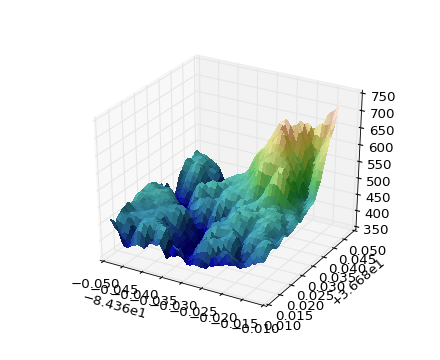
\includegraphics[width=1.1\textwidth]{img/custom_shaded_3d_surface}\\
		\end{minipage}
		\begin{minipage}[c]{0.45\linewidth}
			\centering
			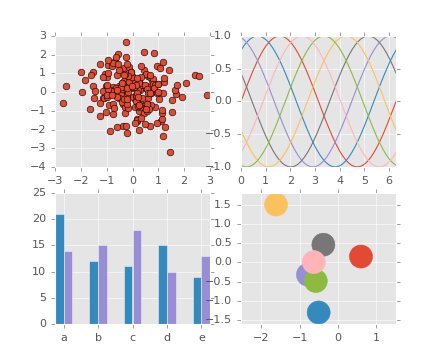
\includegraphics[width=\textwidth]{img/plot-ggplot}\\
			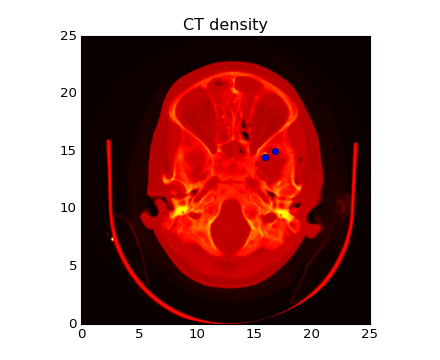
\includegraphics[width=\textwidth]{img/image_demo21}
		\end{minipage}
	\end{figure}
	
\end{frame}

\begin{frame}{Tell me more...}
	\setbeamercovered{invisible}  % to hide from view overlays not yet revealed
	\begin{itemize}
		\item Downloads in the last month (according to PyPI): \alert{\onslide<1>{?}\onslide<2->{180k}}\\
		\item All-time forks on github: \alert{\onslide<1-2>{?}\onslide<3->{1.8k}}\\
		\item All-time contributors to git project: \alert{\onslide<1-3>{?}\onslide<4->{446}}\\
		\item Contributors in the last year: \alert{\onslide<1-4>{?}\onslide<5->{50}}\\
	\end{itemize}
	
	\mynote{As of about April 30, 2016.}
	
\end{frame}

\begin{frame}{Demographics?}
	\mylisthead{Approximate gender breakdown of one year of contributors:}
	\begin{itemize}
		\item Presenting female: \alert{3} 
		\item Gender-neutral: \alert{6}
		\item Presenting male: \alert{41}
	\end{itemize}
	\small{(non-scientific count guessing by gender presented in profile picture or use of a typically gendered name)}
\end{frame}

\begin{frame}{Anatomy of a community}
	\mylisthead{Other than git issues, where is the action at?}\\
	\begin{itemize}
		\item \mylink{Gitter chat room}{http://www.gitter.im/matplotlib/matplotlib}
		\item Mailing list
	\end{itemize}
	\vskip2pt
	\mylisthead{And what other community resources exist?}
	\begin{itemize}
		\item \mylink{Wiki on Github}{https://github.com/matplotlib/matplotlib/wiki}
		\item \mylink{MEPs}{http://matplotlib.org/devel/MEP/index.html}: Matplotlib Enhancement Proposals
		\item \mylink{Developer Guide}{http://matplotlib.org/devel/index.html} (including sections for things like \mylink{Documentation}{http://matplotlib.org/devel/documenting_mpl.html})
		\item \mylink{README}{https://github.com/matplotlib/matplotlib/}, \mylink{INSTALL}{https://github.com/matplotlib/matplotlib/blob/master/INSTALL}
	\end{itemize}
\end{frame}


\begin{frame}{Tonight's project: MEP12}
	\mylink{MEP12}{http://matplotlib.org/devel/MEP/MEP12.html} is a Matplotlib initiative to improve \mylink{this example }{http://matplotlib.org/examples/index.html} \mylink{collection}{http://matplotlib.org/examples/index.html}.	The collection is huge (500 examples!), but not standardized.\\[10pt]
	
	MEP12 sets guidelines for 'cleaning up' examples, and it’s really about improving educational content by making it easier to learn from the examples.  This means doing things like \alert{standardizing style, reorganizing code, and adding comments and descriptions}.
	
	\mylink{Let's look at a cleanup example!}{https://github.com/matplotlib/matplotlib/pull/6303/commits/dcc0d7cc3e8b8185398f2db640c6eec8bc3b6fce}
	
	
\end{frame}

\begin{frame}{Why MEP12?}
	\vskip8pt
	\alert{\textbf{Why choose MEP12 for this hack night?}}
	\begin{itemize}
		\item Examples are isolated, low risk.
		\item They don’t require much domain-specific knowledge.
		\item It’s rewarding: when users come looking for guidance, they'll see your words!
		\item Educational value is something many of us understand.
	\end{itemize}
	
	\vskip10pt
	\alert{\textbf{If it’s so great, why is it still ongoing after 3+ years?}}
	\begin{itemize}
		\item It requires time, thoughtfulness, and subjective judgement calls.
		\item It's non-urgent, easily forgotten when you're busy with bug fixes and new features.
		\item You have to dig into the website to find out it exists, so new contributors might not notice it.
	\end{itemize}
\end{frame}

\section{Hack night instructions}

\begin{frame}
	\centering
	\myunderline{\textbf{Hack night instructions}}
\end{frame}


\begin{frame}{General flow}
	\begin{enumerate}
		\item Follow the steps on the meetup event page!\\[8pt]
		\item Fork matplotlib on github, then clone it to your computer and create a branch.\\[8pt]
		\item Choose an example to work on from the examples folder.  \alert{(Coordinate to avoid collisions! ;))}\\[8pt]
		\item Follow the guidelines on \mylink{MEP12}{http://matplotlib.org/devel/MEP/MEP12.html} and the template on the next slide and edit your example until you're happy with it.  Try to get some feedback from the people around you.\\[8pt]
		\item Pylint your example!  \alert{\texttt{pylint path-to-your-file.py}}\\[8pt]
		\item Commit your code, push to github and make a pull request to matplotlib!
	\end{enumerate}
	

\end{frame}

\begin{frame}{File header template}
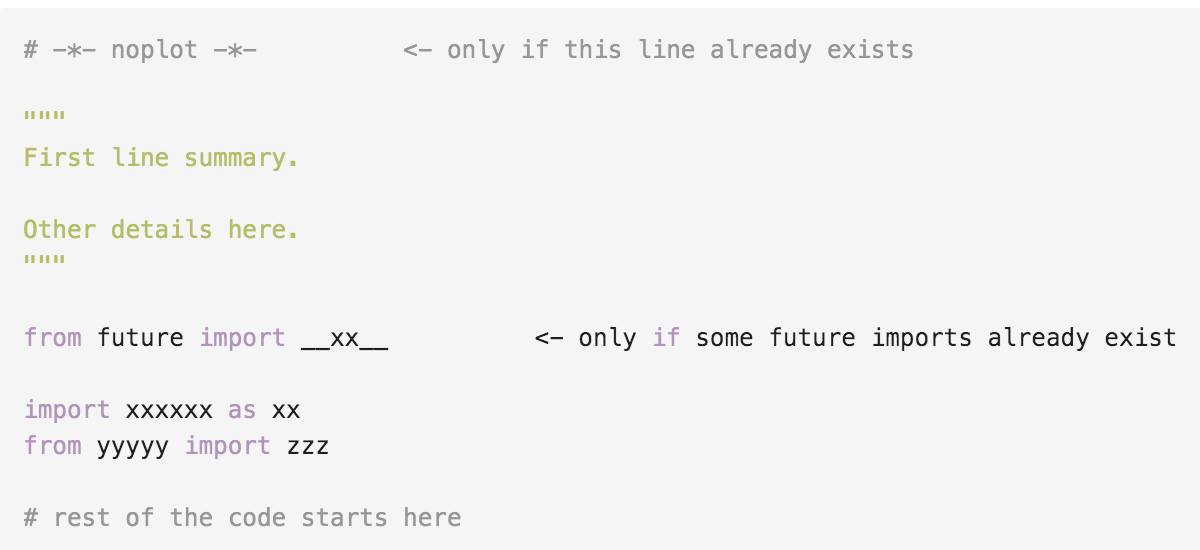
\includegraphics[width=\textwidth]{img/template}\\
\end{frame}




\ThankYouFrame

\end{document}